\let\negmedspace\undefined
\let\negthickspace\undefined
\documentclass[journal]{IEEEtran}
\usepackage[a5paper, margin=10mm, onecolumn]{geometry}
%\usepackage{lmodern} % Ensure lmodern is loaded for pdflatex
\usepackage{tfrupee} % Include tfrupee package

\setlength{\headheight}{1cm} % Set the height of the header box
\setlength{\headsep}{0mm}     % Set the distance between the header box and the top of the text

\usepackage{gvv-book}
\usepackage{gvv}
\usepackage{cite}
\usepackage{amsmath,amssymb,amsfonts,amsthm}
\usepackage{algorithmic}
\usepackage{graphicx}
\usepackage{textcomp}
\usepackage{xcolor}
\usepackage{txfonts}
\usepackage{listings}
\usepackage{enumitem}
\usepackage{mathtools}
\usepackage{gensymb}
\usepackage{comment}
\usepackage[breaklinks=true]{hyperref}
\usepackage{tkz-euclide} 
\usepackage{listings}
% \usepackage{gvv}                                        
\def\inputGnumericTable{}                                 
\usepackage[latin1]{inputenc}                                
\usepackage{color}                                            
\usepackage{array}                                            
\usepackage{longtable}                                       
\usepackage{calc}                                             
\usepackage{multirow}                                         
\usepackage{hhline}                                           
\usepackage{ifthen}                                           
\usepackage{lscape}
\begin{document}

\bibliographystyle{IEEEtran}
\vspace{3cm}

\title{1-1.9-27}
\author{AI24BTECH11028- Ronit Ranjan}

% \maketitle
% \newpage
% \bigskip
{\let\newpage\relax\maketitle}

\renewcommand{\thefigure}{\theenumi}
\renewcommand{\thetable}{\theenumi}
\setlength{\intextsep}{10pt} % Space between text and floats


\numberwithin{equation}{enumi}
\numberwithin{figure}{enumi}
\renewcommand{\thetable}{\theenumi}

\textbf{Question}:\\
If a point A (0, 2) is equidistant from the points B(3, p) and C (p, 5), then find the value of p.


\textbf{Solution}:
We have AB = AC, which implies,
\begin{align}
    \|A-B\| = \|A-C\| \\
    \sqrt{(A-B)^{T}(A-B)} = \sqrt{(A-C)^{T}(A-C)}
\end{align}
where A = \myvec{
0\\
2
}
B = \myvec{
3\\
p
}
C = \myvec{
p\\
5
}.
\begin{align}
    \myvec{
    -3\quad 2-p
    }
    \myvec{
    -3\\
    2-p
    } = 
    \myvec{
    -p\quad -3
    }
    \myvec{
    -p\\
    -3
    }
    \\
    9 + (2-p)^{2} = p^{2} +9 \\
    p = 1
\end{align}
\begin{figure}[hbt!]
		\centering
		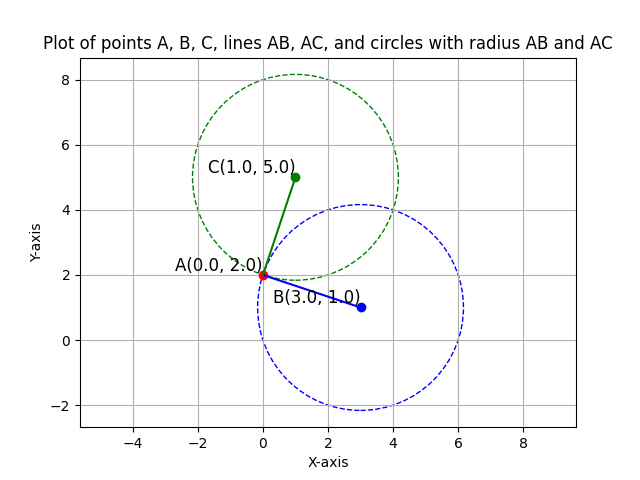
\includegraphics[width=0.8\linewidth]{plots/plot1.png}

	\end{figure}

\end{document}

